\documentclass{article}

\title{\sc\LARGE CSCA67 Tutorial, Week 8\\
{\Large Nov. 2nd-Nov. 6th, 2015}}
\date{}
\author{\sc Compiled by {\em G. Singh Cadieux}\\[1ex]
\sc Adapted from\\
D. Cunningham. \textit{A logical introduction to proof}. Springer, 2012. \&\\
A. Bretscher, \href{http://www.utsc.utoronto.ca/~bretscher/a67/lectures/predicates.pdf}{\em CSCA67 Week 8 Lecture Notes}}

\usepackage{fullpage}
\usepackage{amsmath,amssymb}
\usepackage{color}
%\usepackage{multirow}
\usepackage{tikz}
\usepackage{hyperref}
%\usepackage{array}

\setlength{\parindent}{0pt}

\begin{document}
\maketitle

\section{\sc More formal logic problems}

\subsection*{Q: {\em Show that $(a\vee b)\wedge\neg(a\wedge b)$ is logically equivalent to $a\leftrightarrow \neg b$ using truth tables.}}
Using the method discussed last week, we construct a truth table for each of the statements.\\
(The truth table shown below merges the two truth tables into one.)
\begin{center}
\begin{tabular}{cc|c|c|c|c||c|c}
$a$&$b$&$a\wedge b$&$\neg(a\wedge b)$&$a\vee b$&$(a\vee b)\wedge\neg(a\wedge b)$&$\neg b$&$a\leftrightarrow \neg b$\\\hline
T&T&T&F&T&F&F&F\\
T&F&F&T&T&T&T&T\\
F&T&F&T&T&T&F&T\\
F&F&F&T&F&F&T&F
\end{tabular}
\end{center}
We have shown that the truth table for $(a\vee b)\wedge\neg(a\wedge b)$ and the truth table for $a\leftrightarrow \neg b$ are identical (the truth value of two statements is the same, given the same combination of truth values of $a$ and $b$). Thus, the two statements are logically equivalent.

\subsection*{Q: {\em Construct a truth table for $(p\vee r)\wedge(r\wedge q)$.}}
\begin{center}
\begin{tabular}{ccc|c|c|c}
$p$&$q$&$r$&$p\vee r$&$r\wedge q$&$(p\vee r)\wedge(r\wedge q)$\\\hline
T&T&T&T&T&T\\
T&T&F&T&F&F\\
T&F&T&T&F&F\\
T&F&F&T&F&F\\
F&T&T&T&T&T\\
F&T&F&F&F&F\\
F&F&T&T&F&F\\
F&F&F&F&F&F
\end{tabular}
\end{center}

\subsection*{Q: {\em Shade regions of a Venn diagram where $(p\vee r)\wedge(r\wedge q)$ is true.}}
Let $p$ be the statement ``$x\in P$", $q$ be the statement ``$x\in Q$", and $r$ be the statement ``$x\in R$", where $P,Q,R$ are sets.\\
Then $(p\vee r)\wedge(r\wedge q)$ represents the region(s) of the Venn diagram where $x\in P$ and $x\in Q$, or where $x\in R$ and $x\in Q$.\\[1ex]
Let us first shade in the region where $x\in P$ or $x\in R$ (red). Then let us shade in the region where $x\in R$ and $x\in Q$ (blue). The intersection between these regions represents our statement, since they are joined by an ``and."
\begin{center}
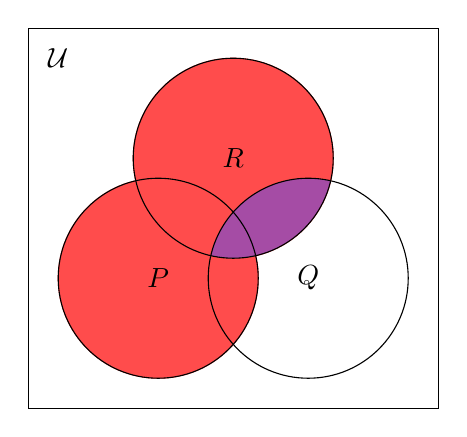
\begin{tikzpicture}
\filldraw[red!70] (0,0) circle[radius=0.5in];
\draw (0.75in,0) circle[radius=0.5in];
\filldraw[red!70] (0.375in,0.6in) circle[radius=0.5in];
\begin{scope}
\path[clip] (0.375in,0.6in) circle[radius=0.5in];
\draw[fill=blue!70,fill opacity=0.5] (0.75in,0) circle[radius=0.5in];
\end{scope}
\draw (-.65in,-.65in) rectangle (1.4in,1.25in);
\draw (0,0) circle[radius=0.5in];
\draw (0.375in,0.6in) circle[radius=0.5in];
\node at (0,0) {$P$};
\node at (0.75in,0) {$Q$};
\node at (0.375in,0.6in) {$R$};
\node at (-.5in,1.1in) {$\mathcal{U}$};
\end{tikzpicture}\qquad
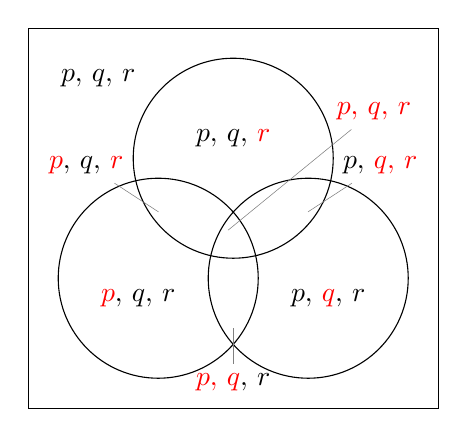
\begin{tikzpicture}[a/.style={pin={[pin distance=.7in]above right:${\color{red}p,\,q,\,r}$}}]
\draw (0,0) circle[radius=0.5in];
\draw (0.75in,0) circle[radius=0.5in];
\draw (0.375in,0.6in) circle[radius=0.5in];
\draw (-.65in,-.65in) rectangle (1.4in,1.25in);
\node at (-.1in,-.1in) {${\color{red}p},\,q,\,r$};
\node at (0.85in,-.1in) {$p,\,{\color{red}q},\,r$};
\node at (0.375in,0.7in) {$p,\,q,\,{\color{red}r}$};
\node at (-.3in,1in) {$p,\,q,\,r$};
\node[pin={above right:$p,\,{\color{red}q,\,r}$}] at (.7in,.3in) {};
\node[pin={above left:${\color{red}p},\,q,\,{\color{red}r}$}] at (.05in,.3in) {};
\node[pin={below:${\color{red}p,\,q},\,r$}] at (.375in,-.2in) {};
\node[a] at (.3in,.2in) {};
\end{tikzpicture}
\end{center}
\textsc{Notice} that the Venn diagram and the truth table for this statement are equivalent. The regions that are shaded in the diagram correspond to the rows of the truth table where the statement is true, and the regions that are not shaded correspond to the rows where the statement is false.

\subsection*{{\normalsize Let $d$ represent ``David likes baseball."\\
Let $j$ represent ``Jaime likes gymnastics."\\
Let $a$ represent ``Anna likes hockey."}\\
Q: {\em Translate each of the following propositions into English.}}
\subsubsection*{a) $\neg d\wedge j\wedge a$}
We start with the most specific statement: $\neg d$ is the negation of ``David likes baseball", which we express in English as ``David does not like baseball".\\[1ex]
Then, $\neg d\wedge j\wedge a$ is the 3-way conjunction (``and") of ``David does not like baseball", ``Jaime likes gymnastics", and ``Anna likes hockey".\\[1ex]
Thus, in English, our statement is ``David does not like baseball and Jaime likes gymnastics and Anna likes hockey".
We might also express this as ``David does not like baseball \textit{but} Jaime likes gymnastics and Anna likes hockey", as well as a number of other sentence structures.

\subsubsection*{b) $\neg (d\wedge j)$}
Again, we start with the most specific statement: $d\wedge j$ is the conjunction of ``David likes baseball" and ``Jaime likes gymnastics", which we express as ``David likes baseball and Jaime likes gymnastics".\\[1ex]
Then, $\neg (d\wedge j)$ is the negation of ``David likes baseball and Jaime likes gymnastics".\\[1ex]
Thus, in English, our statement is ``It is not the case that David likes baseball and Jaime likes gymnastics".
We might express this more naturally as ``David does not like baseball or Jaime does not like gymnastics" (which is really the English translation of an equivalent but different logic statement).

\subsubsection*{c) $\neg d\vee\neg a$}
As above, we translate $\neg d$ to ``David does not like baseball", and similarly, $\neg a$ becomes ``Anna does not like hockey".\\[1ex]
Then, $\neg d\vee\neg a$ is the disjunction (``or") of ``David does not like baseball" and ``Anna does not like hockey".\\[1ex]
Thus, in English, our statement is ``David does not like baseball or Anna does not like hockey".

\subsubsection*{d) $(d\wedge a)\vee j$}
We start with the most specific statement: $d\wedge a$ is the conjunction of ``David likes baseball" and ``Anna likes hockey", which we express in English as ``David likes baseball and Anna likes hockey".\\[1ex]
Then, $(d\wedge a)\vee j$ is the disjunction of ``David likes baseball and Anna likes hockey", and ``Jaime likes gymnastics".\\[1ex]
Thus, in English, our statement is ``David likes baseball and Anna likes hockey, or Jaime likes gymnastics".\\
The comma separating ``David likes [\ldots]" and ``or Jaime likes gymnastics" is meant to indicate that these are two separate clauses of the sentence, so that it is not interpreted as a conjunction of ``David likes baseball" and ``Anna likes hockey, or Jaime likes gymnastics".

\subsection*{Q: {\em Translate each of the following English sentences into formal logic.}}
\subsubsection*{a) ``Jaime doesn't like gymnastics but David likes baseball."}

We start with the most general statement: from the language ``\ldots but\ldots", we know that the statement is a conjunction (``and").\\[1ex]
Then the first part of the conjunction ``Jaime doesn't like gymnastics" is the negation of ``Jaime likes gynmastics".\\[1ex]
Thus, in formal logic, our statement is $\neg j\wedge d$.

\subsubsection*{b) ``Either David likes baseball or Anna likes hockey, and Jaime likes gymnastics."}

Again, we start with the most general statement: from the language ``\ldots and\ldots", we know that the statement is a conjunction.\\[1ex]
Then the first part of the conjunction ``Either David likes baseball or Anna likes hockey" is the disjunction (``or") of ``David likes baseball" and ``Anna likes hockey".\\
However, we must be careful: in English, the use of the word ``either" implies exclusion. The ``$x$ or $y$" we have previously seen is true if $x$ or $y$ or \textit{both} are true (known as ``inclusive or"); this ``either $x$ or $y$" is true if $x$ or $y$ are true, but \textit{not} if both are true.\\
We can express this more clearly as ``David likes baseball and Anna doesn't like hockey, or David doesn't like baseball and Anna likes hockey".\\[1ex]
Thus, in formal logic, our statement is $((d\wedge\neg a)\vee(\neg d\wedge a))\wedge j$.\\[1ex]
Alternatively, because of the ambiguity of the English language, we may consider this statement to be a disjunction of ``David likes baseball" and ``Anna likes hockey, and Jaime likes gymnastics". The comma separating ``Either David likes baseball or Anna likes hockey" and `` and Jaime likes gymnastics" suggests that this is not the case, but it is possible.\\
Then our statement would be $(d\wedge\neg(a\wedge j))\vee(\neg d\wedge(a\wedge j))$.

\subsubsection*{c) ``If Anna likes hockey then David likes baseball."}

From the language ``if\ldots then\ldots", we know that the statement is an implication, with ``Anna likes hockey" as the antecedent (first half) and ``David likes baseball" as the consequent (second half).\\[1ex]
Thus, in formal logic, our statement is $a\to d$.

\section{\sc Predicate Logic}
So far, we have discussed something that we have referred to as ``formal logic." However, we have only studied one branch of formal logic, which we will now properly call \textsc{sentential logic} (also known as ``propositional logic").\\[1ex]
Here, we introduce another branch of formal logic: \textsc{predicate logic}.\\[1em]
Predicate logic addresses some of the limitations of sentential logic:
\begin{itemize}
\item Sentential logic cannot express quantitities/categories, eg. ``\textit{Every} person has a mother," ``\textit{Some} horses are white"
\item Sentential logic cannot express relationships between properties, eg. ``If X is married to Y, then Y is married to X"
\end{itemize}

Predicate logic uses \textsc{predicates} instead of statements/propositions. Predicates are sentences containing variables which can be assigned values. For example, ``$x>5$" is a predicate, where $x$ is the variable.\\[1ex]
Predicates are \textit{not} statements themselves because they have no inherent truth value.\\
\textsc{Consider}: can we say definitively that ``$x>5$" is true or false?\\[1ex]
However, once the variable(s) in the predicate have been assigned values, then the sentence becomes a statement. For example, if we let $x=3$, then ``$x>5$" is a false statement, and if we let $x=6$, then ``$x>5$" is a true statement.

\subsection{\em Syntax}

The language of sentential logic is composed of: sentence symbols, operators/connectives, and parentheses.\\
Since predicate logic uses predicates rather than statements, it uses predicate symbols rather than sentence symbols.\\ Predicate symbols typically follow mathematical function notation, eg. $\overbrace{P(\underbrace{x}_{\text{variable}})}^{\text{predicate}}$.\\
The name of the predicate is typically a single uppercase letter, and the variable is denoted as a single lowercase letter.\\[1ex]
\textsc{Note} that, as with a mathematical function, the letter chosen to represent the variable is simply a placeholder. $P(x)$ is identical to $P(y),\,P(z)$, etc.\\[1em]
We can then use the same connectives as in sentential logic to combine predicates and create compound predicates, eg.
\begin{itemize}
\item $P(x):\,2x=6$
	\begin{itemize}
	\item $P(3)$ is true
	\item $P(10)$ is false
	\end{itemize}
\item $Q(x,y):\,``x\text{ is larger than }y"$
	\begin{itemize}
	\item $Q(\text{Earth},\text{moon})$ is true
	\item $Q(\text{apple},\text{car})$ is false
	\end{itemize}
\item $R(x):\,x<10$
\item $P(x)\wedge R(x)\equiv ``x\text{ is between 5 and 10}"$
	\begin{itemize}
	\item $P(6)\wedge R(6)$ is true
	\item $P(14)\wedge R(14)$ is false
	\end{itemize}
\end{itemize}
\textsc{Note} that, although $x$ is a placeholder, $x$ represents the same value everywhere it is used within a predicate. For example, if we create the compound predicate $P(x)\wedge R(x)$, we cannot assign values such that we have $P(6)\wedge R(14)$.\\[1ex]
Conversely, different variables may represent different values. For example, if we create the compound predicate $P(x)\wedge R(y)$, we \textit{can} assign $x=6$ and $y=14$ such that we have $P(6)\wedge R(14)$.
\begin{itemize}
\item $S(x):\,x<20$
\item $\neg S(x)\equiv ``x$ is greater than or equal to 20"
\item $R(x)\to S(x)\equiv$ ``if $x$ is less than 10, then it is also less than 20"
	\begin{itemize}
	\item $R(3)\to S(3)$ is true
	\item $R(25)\to S(25)$ is (vacuously) true
	\end{itemize}
\end{itemize}
Predicate logic also adds operators called \textsc{quantifiers}, which allow us to describe ranges of values for variables, rather than assigning them individual values.\\[1em]
The \textsc{existential} quantifier is denoted $\exists$ and means ``(there) exists."\\[1ex]
For example, if $P(x):\,``x^2=5"$, then $\exists x(P(x))$ means ``There exists (at least) one value of $x$ for which $x^2=5$". The statement $\exists x(P(x))$ is true, since $P(\sqrt{5})$ and $P(-\sqrt{5})$ are both true.\\[1ex]
If $Q(x):\,``x^2=-5"$, then $\exists x(Q(x))$ means ``There exists (at least) one value of $x$ for which $x^2=-5$", which is false (assuming that $x$ is restricted to the set of reals).\\[1em]
The \textsc{universal} quantifier is denoted $\forall$ and means ``for all/every."\\[1ex]
For example, if $P(x):\,``x^2=5"$, then $\forall x(P(x))$ means ``For every possible value of $x$, $x^2=5$". The statement $\forall x(P(x))$ is false, since only $P(\sqrt{5})$ and $P(-\sqrt{5})$ are true, and $P(x)$ is false for any other value of $x$.\\[1ex]
If $R(x):\,x>5$ and $S(x):\,x>7$, then $\forall x(S(x)\to R(x))$ means ``For every possible value of $x$, if $x$ is greater than 7, $x$ is also greater than 5". We know that this statement is true, since $5<7$ and $7<x$.\\[1em]
As with sentential logic, we may use parentheses to group predicates and operators. When parentheses are omitted, the operators are applied according to the following precedence rules:
\begin{center}
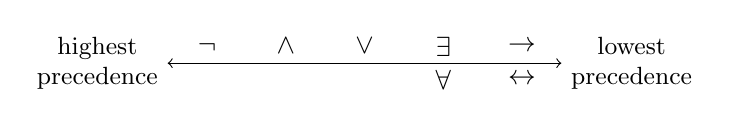
\begin{tikzpicture}
\draw[<->] (0,0) node[left,align=center,font=\small] {highest\\precedence} 
-- (.5,0) node[above] {$\neg$}
-- (1.5,0) node[above] {$\wedge$}
-- (2.5,0) node[above] {$\vee$}
-- (3.5,0) node[align=center] {$\exists$\\$\forall$}
-- (4.5,0) node[align=center] {$\to$\\$\leftrightarrow$}
-- (5,0) node[align=center,right,font=\small] {lowest\\precedence};
\end{tikzpicture}
\end{center}

\subsection{\em Ordering of quantifiers}

When we have a statement containing multiple, different quantifiers, such as $\forall x\exists y(P(x,y))$, the quantified variables are read left to right. For example, if $P(x,y):\,x\cdot y=5$, then $\forall x\exists y(P(x,y))$ means ``For every number $x$, there exists a number $y$ such that $x\cdot y=5$".\\[1ex]
\textsc{Does the} meaning of the sentence change if we reorder the quantifiers?\\
It depends upon the predicate.\\[1ex]
For example, if $P(x,y):\,x>y$, then $\forall x\exists y(P(x,y))$ means ``For every number $x$, there exists a number $y$ such that $x$ is greater than $y$".\\
We know that this statement is true because the set of integers (or reals, depending upon the allowed values of $x$) is infinite. Thus, by definition, there is always a number larger than any number we choose from the set.\\[1ex]
But $\exists y\forall x(P(x,y))$ means ``There exists a number $y$ such that, for every number $x$, $x$ is greater than $y$".\\
We know that this statement is false because it is saying that there is some minimum integer (since every other integer is larger than it). Since the integers are infinite, this is impossible.\\[1ex]
Here, the order of the quantifiers is significant.

\subsection{\em Negation of quantifiers}

In addition to negating predicates using the negation operator, we want to be able to negate quantifiers - that is, we want to be able to say ``There does \textit{not} exist\ldots" and ``\textit{It is not the case that} for all\ldots".\\[1ex]
For some predicate $P(x)$, ``There does \textit{not} exist an $x$ such that $P(x)$ is true" is equivalent to saying ``$P(x)$ is false for every value of $x$", which we can write formally as $\forall x(\neg P(x))$.\\[1ex]
For some predicate $P(x)$, ``\textit{It is not the case that}, for every value of $x$, $P(x)$ is true" is equivalent to saying ``There is some value of $x$ for which $P(x)$ is false", which we can write formally as $\exists x(\neg P(x))$.\\[1ex]
Thus, the negation of $\exists x(P(x))$ is $\forall x(\neg P(x))$ and the negation of $\forall x(P(x))$ is $\exists x(\neg P(x))$.\\[1em]
For example, if $P(x)$: ``$x$ is tall", where $x$ is a person, then
\begin{itemize}
\item $\exists x(P(x))$ means ``There exists a person who is tall"
\item $\forall x(\neg(P(x))$ means ``Every person is not tall", or ``There does not exist a person who is tall"
\item $\forall x(P(x))$ means ``All people are tall"
\item $\exists x(\neg P(x))$ means ``There exists a person who is not tall", or ``Not every person is tall"
\end{itemize}

\section{\sc Additional practice problems}
Let $P(x,y)$ be the predicate ``$x\cdot y=12$", where $x,y$ are integers.\\
{\bf Q: Which of the following statements is true?}
\begin{itemize}
\item $P(3,4)$
\item $P(3,5)$
\item $P(2,6)\vee P(3,7)$
\item $\forall x,\forall y(P(x,y)\to P(y,x))$
\item $\forall x,\exists y(P(x,y))$
\end{itemize}
\vspace{1ex}Given the predicates\\
$L(x)=$``$x$ is a lion."\\
$F(x)=$``$x$ is fuzzy."\\
where $x$ is a mammal,\\
{\bf Q: Translate ``All lions are fuzzy" into predicate logic.}\\[1ex]
{\bf Q: Translate ``Some lions are fuzzy" into predicate logic.}\\[1em]
Consider the three predicates\\
$P(x)$ symbolizes the statement ``$x$ is a prime number"\\
$E(x)$ symbolizes the statement ``$x$ is even"\\
$D(x, y)$ symbolizes the statement ``$x$ evenly divides $y$"\\
where $x$ and $y$ represent integers.\\
{\bf Q: Find some values for the variables that make the following logical formulas true, and others making them false.}
\begin{itemize}
\item $P(x) \wedge E(x)$
\item $E(x) \vee D(x, y)$
\item $\neg P(x) \wedge D(x, y)$
\item $D(x, y) \to\neg P(x)$
\end{itemize}
\vspace{1ex}\textit{Tarski's World} is a computer program that is meant to be an introduction to predicate logic.\\
You can build two-dimensional worlds of shapes, describe them using predicates, and test whether your predicates are true or false.\\
Experiment with Tarski's World using the following implementation: \href{http://courses.cs.washington.edu/courses/cse590d/03sp/tarski/tarski.html}{Tarski's World (Java Applet)}

\end{document}